\documentclass[10pt]{article}
% Layout mirrors the NeurIPS template (5.5in x 9in text block, Times).
% Before submission, replace this preamble with the official neurips_2026.sty.
\usepackage[letterpaper,textwidth=5.5in,textheight=9in,top=1in]{geometry}
\usepackage[T1]{fontenc}
\usepackage{newtxtext,newtxmath}
\usepackage{graphicx,booktabs,amsmath,xcolor,microtype}
\usepackage[numbers,sort&compress]{natbib}
\usepackage[colorlinks,linkcolor=blue!50!black,citecolor=blue!50!black,urlcolor=blue!50!black]{hyperref}
\usepackage{caption}
\captionsetup{font=small,labelfont=bf}
\setlength{\emergencystretch}{1.5em}
% Generated by paper/make_numbers.py from results/*.json. Do not edit.
\newcommand{\AliveRatioTwo}{1.74}
\newcommand{\BootN}{60}
\newcommand{\ChaoRatioEq}{39\times}
\newcommand{\ChaoRatioMax}{28{,}303\times}
\newcommand{\HeldHierBigNoGrowthMax}{7.3\%}
\newcommand{\HeldHierBigNoGrowthMed}{3.5\%}
\newcommand{\HeldHierBigSfMax}{16.5\%}
\newcommand{\HeldHierBigSfMed}{7.4\%}
\newcommand{\HeldHierSmallNoGrowthMax}{9.1\%}
\newcommand{\HeldHierSmallNoGrowthMed}{6.7\%}
\newcommand{\HeldHierSmallSfMax}{14.8\%}
\newcommand{\HeldHierSmallSfMed}{13.6\%}
\newcommand{\HeldRealMZeroMax}{30.4\%}
\newcommand{\HeldRealMZeroMed}{29.8\%}
\newcommand{\HeldRealNoGrowthMax}{38.5\%}
\newcommand{\HeldRealNoGrowthMed}{37.0\%}
\newcommand{\HeldRealSfMax}{4.3\%}
\newcommand{\HeldRealSfMed}{1.4\%}
\newcommand{\HeldSynBigMZeroMax}{0.4\%}
\newcommand{\HeldSynBigMZeroMed}{0.2\%}
\newcommand{\HeldSynBigN}{9}
\newcommand{\HeldSynBigNoGrowthMax}{0.4\%}
\newcommand{\HeldSynBigNoGrowthMed}{0.3\%}
\newcommand{\HeldSynBigSfMax}{9.2\%}
\newcommand{\HeldSynBigSfMed}{0.3\%}
\newcommand{\HeldSynSmallMZeroMax}{13.6\%}
\newcommand{\HeldSynSmallMZeroMed}{10.6\%}
\newcommand{\HeldSynSmallN}{8}
\newcommand{\HeldSynSmallNoGrowthMax}{14.2\%}
\newcommand{\HeldSynSmallNoGrowthMed}{10.9\%}
\newcommand{\HeldSynSmallSfMax}{10.2\%}
\newcommand{\HeldSynSmallSfMed}{6.8\%}
\newcommand{\HierC}{4}
\newcommand{\HierChildren}{1{,}024}
\newcommand{\HierDiverged}{0}
\newcommand{\HierDraws}{2}
\newcommand{\HierJunkSingle}{93\%}
\newcommand{\HierKidsDouble}{1{,}024}
\newcommand{\HierKidsEighth}{102}
\newcommand{\HierKidsFull}{1{,}024}
\newcommand{\HierKidsHalf}{650}
\newcommand{\HierKidsQuarter}{262}
\newcommand{\HierMMax}{2{,}048}
\newcommand{\HierMMin}{128}
\newcommand{\HierParentCos}{0.72}
\newcommand{\HierParents}{256}
\newcommand{\HierParsDouble}{6}
\newcommand{\HierParsEighth}{76}
\newcommand{\HierParsFull}{138}
\newcommand{\HierParsHalf}{220}
\newcommand{\HierParsQuarter}{157}
\newcommand{\HierReachDouble}{1{,}030}
\newcommand{\HierReachEighth}{178}
\newcommand{\HierReachFull}{1{,}162}
\newcommand{\HierReachHalf}{870}
\newcommand{\HierReachQuarter}{420}
\newcommand{\HierRuns}{80}
\newcommand{\HierSfDouble}{1{,}030}
\newcommand{\HierSfEighth}{154}
\newcommand{\HierSfErrDouble}{1.5\%}
\newcommand{\HierSfErrFull}{11.3\%}
\newcommand{\HierSfFull}{909}
\newcommand{\HierSfFullTauHi}{1{,}197}
\newcommand{\HierSfFullTauLo}{828}
\newcommand{\HierSfHalf}{615}
\newcommand{\HierSfQuarter}{308}
\newcommand{\HierSfReachMax}{0.94}
\newcommand{\HierSfReachMed}{0.73}
\newcommand{\HierSfReachMin}{0.70}
\newcommand{\HierSiblingCos}{0.36}
\newcommand{\HierUnionDouble}{6{,}855}
\newcommand{\HierUnionEighth}{188}
\newcommand{\HierUnionFull}{1{,}544}
\newcommand{\HierUnionHalf}{705}
\newcommand{\HierUnionQuarter}{374}
\newcommand{\HierUnionRatioMax}{6.7}
\newcommand{\JunkMultiMax}{0\%}
\newcommand{\JunkSingleEq}{93\%}
\newcommand{\JunkSingleOver}{92\%}
\newcommand{\MainTau}{0.8}
\newcommand{\NComplete}{9}
\newcommand{\NEstimators}{11}
\newcommand{\NIncomplete}{8}
\newcommand{\OracleUnionHalf}{71\%}
\newcommand{\OracleUnionQuarter}{31\%}
\newcommand{\PlateauMed}{1.02}
\newcommand{\RealAllSeedsEight}{308}
\newcommand{\RealAllSeedsTwo}{167}
\newcommand{\RealChoiceEight}{mix3}
\newcommand{\RealChoiceFour}{mix3}
\newcommand{\RealChoiceOne}{mix3}
\newcommand{\RealChoiceTwo}{mix3}
\newcommand{\RealEvalTokens}{65{,}536}
\newcommand{\RealFvuEight}{0.073}
\newcommand{\RealFvuFour}{0.077}
\newcommand{\RealFvuOne}{0.090}
\newcommand{\RealFvuTwo}{0.082}
\newcommand{\RealGrowthFour}{1.26}
\newcommand{\RealGrowthOne}{1.86}
\newcommand{\RealGrowthTwo}{1.56}
\newcommand{\RealK}{32}
\newcommand{\RealLayer}{3}
\newcommand{\RealLongAllSeeds}{384}
\newcommand{\RealLongFvu}{0.072}
\newcommand{\RealLongHeldErr}{0.4\%}
\newcommand{\RealLongRatio}{1.27}
\newcommand{\RealLongSeenTwo}{1{,}559}
\newcommand{\RealLongSf}{2{,}054}
\newcommand{\RealLongSfHi}{2{,}472}
\newcommand{\RealLongSfLo}{1{,}868}
\newcommand{\RealLongStepRatio}{2.5}
\newcommand{\RealLongTauMax}{2{,}079}
\newcommand{\RealLongTauMin}{1{,}732}
\newcommand{\RealLongTokens}{10{,}000{,}000}
\newcommand{\RealReproFrac}{39\%}
\newcommand{\RealSeeds}{8}
\newcommand{\RealSeenTwoEight}{1{,}867}
\newcommand{\RealSeenTwoFour}{1{,}428}
\newcommand{\RealSeenTwoOne}{543}
\newcommand{\RealSeenTwoTwo}{934}
\newcommand{\RealSfEight}{3{,}172}
\newcommand{\RealSfEightKFour}{2{,}695}
\newcommand{\RealSfEightKSix}{3{,}268}
\newcommand{\RealSfEightTauHi}{1{,}238}
\newcommand{\RealSfEightTauLo}{4{,}254}
\newcommand{\RealSfFour}{2{,}520}
\newcommand{\RealSfFourTauHi}{1{,}543}
\newcommand{\RealSfFourTauLo}{2{,}967}
\newcommand{\RealSfHiEight}{3{,}952}
\newcommand{\RealSfHiFour}{2{,}941}
\newcommand{\RealSfHiOne}{1{,}083}
\newcommand{\RealSfHiTwo}{2{,}011}
\newcommand{\RealSfLoEight}{2{,}869}
\newcommand{\RealSfLoFour}{2{,}113}
\newcommand{\RealSfLoOne}{728}
\newcommand{\RealSfLoTwo}{1{,}303}
\newcommand{\RealSfOne}{870}
\newcommand{\RealSfOneTauHi}{673}
\newcommand{\RealSfOneTauLo}{991}
\newcommand{\RealSfTwo}{1{,}616}
\newcommand{\RealSfTwoTauHi}{1{,}123}
\newcommand{\RealSfTwoTauLo}{1{,}543}
\newcommand{\RealSingleFrac}{97\%}
\newcommand{\RealTrainTokens}{2{,}000{,}000}
\newcommand{\RealTwoTauMax}{1{,}616}
\newcommand{\RealTwoTauMin}{1{,}123}
\newcommand{\RealUnionEight}{57{,}614}
\newcommand{\RealUnionFour}{27{,}515}
\newcommand{\RealUnionGrowth}{9.4}
\newcommand{\RealUnionOne}{6{,}107}
\newcommand{\RealUnionTwo}{12{,}900}
\newcommand{\SfDivComplete}{0}
\newcommand{\SfDivIncomplete}{0}
\newcommand{\SfMaxErrComplete}{3.2\%}
\newcommand{\SfMaxErrCompleteHalfPmin}{7.1\%}
\newcommand{\SfMaxErrCompleteTauHi}{5.7\%}
\newcommand{\SfMaxErrCompleteTauLo}{7.7\%}
\newcommand{\SfReachHi}{1.19}
\newcommand{\SfReachLo}{0.86}
\newcommand{\SfReachMed}{0.95}
\newcommand{\SynAlpha}{0.7}
\newcommand{\SynD}{128}
\newcommand{\SynFamilies}{17}
\newcommand{\SynK}{8}
\newcommand{\SynMeanActive}{5}
\newcommand{\SynRuns}{136}
\newcommand{\SynSeeds}{8}
\newcommand{\SynSteps}{1{,}200}
\newcommand{\TauHi}{0.9}
\newcommand{\TauLo}{0.7}
\newcommand{\UnionRatioEq}{1.47}
\newcommand{\UnionRatioMax}{12.2}


\title{Counting Fish in the Residual Stream:\\Capture--Recapture Estimates of How Many Features a Sparse Autoencoder Can Find}
\author{Anonymous Author(s)}
\date{}

\begin{document}
\maketitle

\begin{abstract}
How many features does a language model have? Sparse autoencoders (SAEs) split a model's activations into features, but their dictionary size is chosen by hand, and SAEs trained with different random seeds find different features. We turn that seed disagreement into a census using capture--recapture, the method ecologists use to count animals they cannot see all at once. Each seed is a net, and a feature that several seeds find is a recaptured animal.

We first test this on synthetic activations with a known, planted number of features. Every naive count errs in the same direction. The number of distinct features across seeds overstates the truth by up to \UnionRatioMax-fold, and Chao's classical estimator by up to $\ChaoRatioMax$. The cause is seed-specific junk latents, which pose as rare features caught once, much as sequencing errors create false species in microbial surveys. A \emph{singleton-free} estimator fits a bounded catch-probability mixture only to features that at least two seeds find. Whenever the dictionary is large enough, it lands within \SfMaxErrComplete{} of the planted count. As the dictionary grows further it levels off at that count while the naive counts keep rising. When planted features split into finer ones, it levels off at the finest level once the dictionary can hold it, and undercounts by \HierSfErrFull{} when the dictionary is just large enough.

On Pythia-70M, the estimated number of reproducible features grows, more and more slowly, from \RealSfOne{} at 1k latents to \RealSfEight{} at 8k, against \RealUnionEight{} distinct latents across seeds. Fitted on four seeds, the estimator predicts how many features eight seeds will reproduce to within \HeldRealSfMax. Assuming no new features would appear misses by a median of \HeldRealNoGrowthMed. Training on five times more data raises the count by a factor of \RealLongRatio{}, so these numbers are lower bounds. The census also depends on how strictly two latents must match to count as the same feature, and we report that dependence. Everything reruns on a laptop CPU.
\end{abstract}

\section{Introduction}
\label{sec:intro}

How many fish live in a lake? You cannot drain it to count them. Ecologists catch a net-full, tag each fish, and release them. A week later they catch another net-full and count how many carry tags. If a tenth of the second catch is tagged, the first catch was about a tenth of the lake. This is the capture--recapture method. Variants of it estimate wildlife populations, the number of species in a soil sample, and the number of people a census missed \citep{chao1987estimating,fienberg1972multiple,colwell2012models}.

Interpretability researchers face the same problem inside neural networks. A sparse autoencoder (SAE) rewrites a model's internal activations as a sparse combination of directions, called \emph{features}, many of which correspond to human-recognisable concepts \citep{cunningham2023sparse,bricken2023monosemanticity,templeton2024scaling}. A basic question has no accepted answer: \emph{how many features does a model have?} Dictionary size is chosen by hand. Larger dictionaries keep finding new latents \citep{gao2024scaling}. SAEs trained twice on the same data with different random seeds find partly different features \citep{paulo2025sparse}. Seed disagreement is usually treated as a nuisance.

We treat it as data. Each SAE seed is one net cast into the same lake. A feature found by several seeds has been recaptured, and a feature found by one seed was caught once. Whether some features are never found becomes a statistical question, the one capture--recapture answers. The analogy has one twist with no counterpart in fish. An SAE sometimes learns a direction that no other seed reproduces and that corresponds to no real feature. Ecologists know this failure from DNA-based surveys, where sequencing errors create ``species'' seen exactly once \citep{chiu2016estimating}.

\paragraph{Contributions.}
\begin{enumerate}\setlength\itemsep{1pt}
\item \textbf{A census method for features.} We cast SAE seed (dis)agreement as closed-population capture--recapture. We compare \NEstimators{} counts and estimators from ecology and statistics against planted ground truth, across \SynFamilies{} synthetic settings and \SynRuns{} trained SAEs (\S\ref{sec:method}).
\item \textbf{Naive counts fail, in a predictable direction.} Counting distinct features across seeds overstates the planted count by a median factor of \UnionRatioEq{} when the dictionary has as many latents as there are features, and by up to \UnionRatioMax$\times$ when it has more. Chao's classical estimator overstates it by up to $\ChaoRatioMax$. The cause is seed-specific junk latents: \JunkSingleOver{} of features caught once are junk when the dictionary is larger than the feature count (\S\ref{sec:results}).
\item \textbf{A singleton-free estimator that recovers the planted count.} It fits a bounded catch-probability mixture to features found by at least two seeds. Whenever the dictionary is at least as large as the true count, it is within \SfMaxErrComplete{} of the truth in all \NComplete{} settings. When the dictionary is too small, it tracks the features a dictionary of that size can reach, not the truth, so its rise and \emph{plateau} across dictionary sizes reveal the feature count. When planted features split into finer ones, the plateau appears only once the dictionary can hold the finest level (\S\ref{sec:hier}). It also predicts what held-out seeds will find.
\item \textbf{A census of Pythia-70M.} In the residual stream of Pythia-70M \citep{biderman2023pythia}, the estimated number of reproducible features grows from \RealSfOne{} to \RealSfEight{} as the dictionary grows from 1k to 8k latents, and growth slows without stopping. Fitted on four seeds, the census predicts what eight seeds reproduce to within \HeldRealSfMax. Five times more training data raises the count by a factor of \RealLongRatio{}, so all of these counts are lower bounds (\S\ref{sec:real}).
\end{enumerate}

\section{Related work}
\label{sec:related}

\paragraph{How many features?} Sparse autoencoders decompose activations into an overcomplete dictionary of sparsely active directions \citep{sharkey2022interim,cunningham2023sparse,bricken2023monosemanticity}. Dictionary size is a free choice. Larger dictionaries keep lowering reconstruction error along a power law \citep{gao2024scaling,templeton2024scaling}, and they split coarse features into finer ones \citep{bricken2023monosemanticity}. Meta-SAEs and stitching show that features are not atomic units \citep{leask2025sparse}. \citet{engels2024decomposing} study the reconstruction error SAEs leave unexplained (``dark matter''), and the quantization model of scaling posits a discrete set of skills with power-law frequencies \citep{michaud2023quantization}. None of these estimates the number of features a model has from data. Loss-curve extrapolations predict reconstruction error, not counts.

\paragraph{Seed (dis)agreement.} \citet{paulo2025sparse} found that SAEs trained on the same data with different seeds share only part of their latents, and that the shared fraction depends on architecture and size. Cross-model studies compare SAE feature spaces between language models \citep{lan2024sparse}. These works treat disagreement as a reliability problem. We treat it as data. The pattern of which seeds find which feature is exactly the capture history that population ecologists use to count animals they cannot see all at once.

\paragraph{Capture--recapture and unseen species.} Estimating a closed population from repeated incomplete samples goes back to Petersen and Lincoln. Its modern forms include Chapman's correction \citep{chapman1951some}, multiple-occasion models \citep{darroch1958multiple,otis1978statistical}, log-linear multiple-systems estimation \citep{fienberg1972multiple}, Chao's estimators for unequal catchability \citep{chao1987estimating}, jackknives \citep{burnham1978estimation}, and mixture models \citep{pledger2000unified,dorazio2003mixture}, with the caveat that heterogeneous populations are not identifiable without assumptions \citep{link2003nonidentifiability}. The incidence-based rarefaction and extrapolation framework \citep{colwell2012models} supplies the seed-accumulation curves we use. In machine learning, Good--Turing estimation \citep{good1953population} has been used to extrapolate how much training data a language model has memorised \citep{nasr2023scalable}. We know of no prior application of capture--recapture to learned features, and the misidentification problem it raises connects to work on sequencing-error singletons in microbial ecology \citep{chiu2016estimating}.

\section{Method}
\label{sec:method}

\subsection{Seeds as capture occasions}
We train $K$ sparse autoencoders on the same activations, in the same order, changing only the random seed of the initialisation, which is the setting in which \citet{paulo2025sparse} found that seeds disagree. Each SAE is one \emph{capture occasion}. A latent is \emph{alive} if it fires on at least $10^{-5}$ of held-out tokens, and it is represented by its unit-norm decoder direction. A \emph{species} is a feature, and the data of the survey is the \emph{capture history} matrix $H\in\{0,1\}^{S\times K}$, where $H_{sr}=1$ when run $r$ contains a latent for species $s$ and $S$ is the number of species seen at least once. Species that no run caught are, by construction, absent from $H$. Estimating how many of them there are is the problem.

\paragraph{Identifying individuals.} An ecologist recognises a recaptured fish by its tag. We need a rule that decides when latents of two runs are the same feature.
\begin{itemize}\setlength\itemsep{0pt}
\item \emph{Oracle} identification (synthetic data only): run $r$ catches planted feature $i$ if one of its alive latents has cosine similarity $\ge\tau$ with $f_i$.
\item \emph{Blind} identification (no ground truth): for every pair of runs, two latents are linked if they are mutual nearest neighbours with decoder cosine $\ge\tau$. Connected components of the resulting graph are species.
\end{itemize}
We use $\tau=\MainTau$ throughout and report $\tau\in\{\TauLo,\TauHi\}$ as robustness checks.

\subsection{Estimators}
Let $Q_j$ be the number of species caught on exactly $j$ of the $K$ occasions, so that $S=\sum_{j\ge1}Q_j$. We compare four families.

\emph{Naive counts.} These are the dictionary size $m$, the number of alive latents in one SAE, and the union $S$ over all seeds, which is the strongest simple baseline because it counts every distinct feature any seed found. We also fit the Michaelis--Menten curve $S(t)=at/(b+t)$ to the seed-accumulation (rarefaction) curve and report its asymptote $a$ \citep{raaijmakers1987statistical,colwell2012models}.

\emph{Equal-catchability models.} These are Chapman's bias-corrected Lincoln--Petersen estimator \citep{chapman1951some}, averaged over all pairs of seeds, and the maximum-likelihood estimator for model $M_t$ \citep{darroch1958multiple}. Both assume every feature is equally easy to catch.

\emph{Heterogeneous-catchability models} (model $M_h$ \citep{otis1978statistical}). These are Chao's lower bound $\hat N=S+\tfrac{K-1}{K}\,Q_1^2/(2Q_2)$ \citep{chao1987estimating}, the first- and second-order jackknives \citep{burnham1978estimation}, and a beta-binomial mixture fitted by maximum likelihood to all observed species \citep{dorazio2003mixture}. Rare features fire on few tokens and contribute little to reconstruction loss, so they are caught less often. That is exactly the heterogeneity these models were built for.

\emph{Singleton-free mixtures} (our adaptation). Blind identification has a failure that tagging does not: a latent that no other seed reproduces becomes a species caught once, whether it is a real but rare feature or seed-specific noise. Microbial ecologists meet the same problem when sequencing errors create spurious singletons that inflate Chao-type estimates \citep{chiu2016estimating}. We therefore fit a catchability mixture only to $Q_2,\dots,Q_K$, the species seen at least twice, by maximising the zero- and one-truncated likelihood. The estimate is $\hat N=S_{\ge2}/\hat P(Y\ge2)$, where $Y$ is the number of seeds that catch a feature. The mixing distribution is a mixture of one to three binomial classes \citep{pledger2000unified}, chosen by AIC, with every class's catch probability bounded below by $p_{\min}=1/K$.

The bound defines what is counted: features that $K$ seeds find at least once on average. It is also what makes the estimate finite. Without it the truncated likelihood barely changes when mass is moved toward $p=0$, so a few stray recaptures can send $\hat N$ to infinity \citep{link2003nonidentifiability}. We call this estimator \emph{singleton-free} and report the unbounded beta-binomial and two-class versions as ablations.

\paragraph{Uncertainty.} Confidence intervals are 95\% percentile intervals from \BootN{} Chao-style bootstrap resamples. We pad $H$ with $\hat N-S$ all-zero histories, resample species with replacement, and re-estimate. Population size under arbitrary heterogeneity is not identifiable \citep{link2003nonidentifiability}: features that no SAE of a given size will ever catch leave no trace. The estimators therefore target features an SAE family can reach, and the synthetic experiments measure how close that is to the truth.

\subsection{Synthetic activations with a planted answer}
Activations are $x=\sum_i a_i f_i$, with $N$ random unit features $f_i\in\mathbb R^{\SynD}$. Feature $i$ is active independently with probability $p_i\propto i^{-\SynAlpha}$, scaled so that \SynMeanActive{} features are active on average, and has magnitude $a_i\sim U(0.5,1.5)$. Planted counts are $N\in\{512,1024,2048\}$, so features outnumber dimensions by a factor of 4--16, the superposition regime \citep{elhage2022toy}. We train TopK SAEs \citep{gao2024scaling} with $k=\SynK$ and dictionary sizes from $N/4$ to $4N$ (capped at 4096), $K=\SynSeeds$ seeds each, for \SynSteps{} steps of 4096 samples (three passes over a fixed set of 1.6M samples). Training uses Adam (learning rate $2\times10^{-3}$, linear decay over the last 20\%), unit-norm decoder rows, and the AuxK loss for dead latents. A second draw of features and data repeats the $N=1024$ sweep.

\subsection{Pythia-70M}
We cache the residual stream after block \RealLayer{} of Pythia-70M \citep{biderman2023pythia} on \RealTrainTokens{} training tokens from 128-token contexts of the Pile \citep{gao2020pile}, using documents 500 onward of the public \texttt{pile-10k} sample. Evaluation uses \RealEvalTokens{} tokens from documents 0--499. The first position of each context is dropped, and activations are scaled so that $\mathbb E\|x\|^2=d$. SAEs use $k=\RealK$, $m\in\{1024,2048,4096,8192\}$, two passes over the data, and $K=\RealSeeds$ seeds per size.

\section{Results}
\label{sec:results}

\begin{figure}[t]
\centering
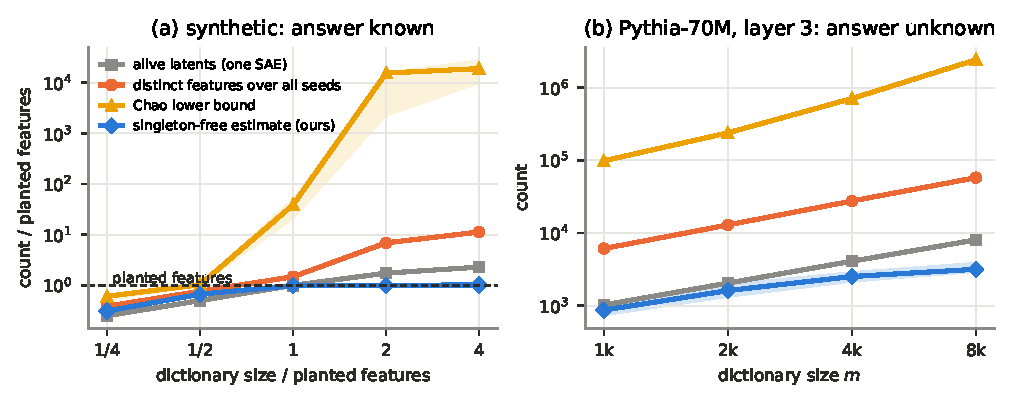
\includegraphics[width=\linewidth]{../figures/fig1_hero.pdf}
\caption{\textbf{Counting features with a fish-counting method.} (a) Synthetic activations with a known number $N$ of planted features (\SynFamilies{} settings; lines are medians, bands the range across settings). As the dictionary grows, the number of alive latents (gray) and the number of distinct features found across \SynSeeds{} seeds (orange) keep rising, and Chao's estimator (yellow) explodes. The singleton-free capture--recapture estimate (blue) rises until the dictionary is large enough and then levels off at the planted count (dashed). (b) The same quantities for Pythia-70M, where the true count is unknown. The blue band is the 95\% bootstrap interval.}
\label{fig:hero}
\end{figure}

\subsection{Naive counts overstate the number of features}
Table~\ref{tab:synth} and Figure~\ref{fig:hero}a compare every count and estimator with the planted number $N$. Once the dictionary has at least as many latents as there are planted features, every naive count is too high, and the error grows with the dictionary.
\begin{itemize}\setlength\itemsep{1pt}
\item \emph{Alive latents in one SAE:} \AliveRatioTwo$N$ at $m=2N$.
\item \emph{Distinct features across all seeds:} \UnionRatioEq$N$ at $m=N$ (median), and up to \UnionRatioMax$N$ at $m=4N$.
\item \emph{Equal-catchability estimators} (Lincoln--Petersen, $M_t$) and the Michaelis--Menten curve inherit the same inflation.
\item \emph{Heterogeneity estimators} built for exactly this kind of data are the worst. Chao's bound is $\ChaoRatioEq$ the truth at $m=N$ and up to $\ChaoRatioMax$ beyond, and the jackknife is also too high, increasingly so as the dictionary grows. The beta-binomial fitted to all species diverges in every setting.
\end{itemize}

\begin{table}[t]
\centering\small
\caption{\textbf{Estimated count divided by the planted count $N$} (median over settings; blind matching, $\tau=\MainTau$; \SynSeeds{} seeds). A superscript gives the number of settings in which the estimate diverged ($\hat N>10^9$), and ``div.'' means it diverged in every setting. The last two rows use the ground truth and are not available in practice. ``Reachable'' is the number of planted features that at least one seed caught.}
\label{tab:synth}
\begin{tabular}{lrrrrr}
\toprule
estimator & \multicolumn{5}{c}{dictionary size $m$} \\
 & $N/4$ & $N/2$ & $N$ & $2N$ & $4N$ \\
\midrule
alive latents (one SAE) & 0.25 & 0.50 & 1.00 & 1.74 & 2.28 \\
distinct features, all seeds & 0.38 & 0.76 & 1.47 & 6.88 & 11 \\
Michaelis--Menten asymptote & 0.40 & 0.80 & 1.49 & 18 & 46 \\
Lincoln--Petersen (Chapman) & 0.29 & 0.58 & 1.11 & 3.01 & 5.22 \\
Darroch $M_t$ & 0.38 & 0.76 & 1.47 & 8.02 & 16 \\
Chao $M_h$ bound & 0.61 & 1.03 & 39 & 15{,}470 & 18{,}962 \\
jackknife (2nd order) & 0.55 & 1.04 & 2.26 & 16 & 28 \\
beta-binomial, all species & div. & div. & div. & div. & div. \\
\quad singletons dropped, unbounded & 0.40$^{(3)}$ & 5.85$^{(3)}$ & 0.98 & div. & div. \\
two-class, singletons dropped, unbounded & 0.29 & 0.59 & 0.98 & 1.00$^{(1)}$ & 1.01 \\
\textbf{singleton-free (ours)} & 0.31 & 0.67 & 0.98 & 1.00 & 1.01 \\
singleton-free, oracle IDs & 0.28 & 0.67 & 1.00 & 1.00 & 1.00 \\
oracle: reachable (union, oracle IDs) & 0.31 & 0.71 & 1.00 & 1.00 & 1.00 \\
\bottomrule
\end{tabular}

\end{table}

\subsection{Why: junk latents are caught once}
Figure~\ref{fig:mechanism}a shows the capture frequencies behind these failures. Blind matching produces a spike of features caught by a single seed. At $m=N$, \JunkSingleEq{} of those singletons match no planted feature (median over settings), and at $m>N$ the figure is \JunkSingleOver. They are directions that one seed learned and no other seed reproduced, the analogue of sequencing-error ``species'' in microbial surveys \citep{chiu2016estimating}. Features seen by two or more seeds are almost all real: across frequency classes with at least 20 features, the largest junk fraction is \JunkMultiMax{} when $m\ge N$. Chao's bound grows with the square of the singleton count, which explains its explosion. Capture probabilities are also genuinely unequal (Figure~\ref{fig:mechanism}b). When the dictionary is too small, the rarest features are caught by few seeds or none, the heterogeneity that model $M_h$ describes \citep{otis1978statistical}.

\begin{figure}[t]
\centering
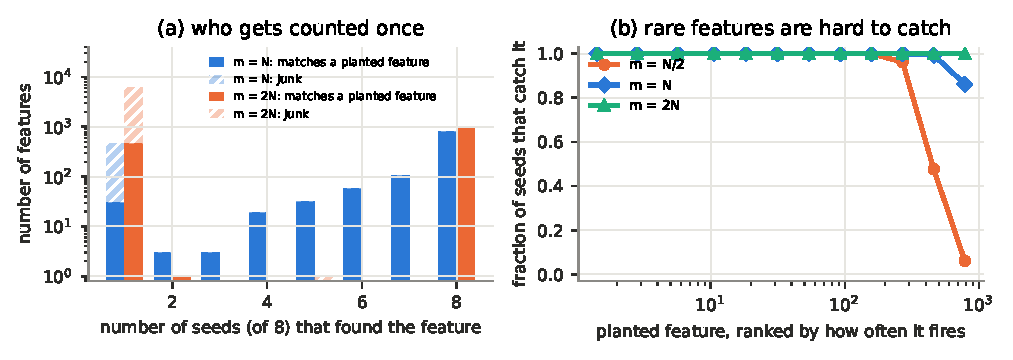
\includegraphics[width=\linewidth]{../figures/fig2_mechanism.pdf}
\caption{\textbf{Where naive counts go wrong} ($N=1024$, first data draw). (a) How many of the \SynSeeds{} seeds found each feature, under blind matching. Hatched bar segments match no planted feature. Almost all of them sit at ``found by one seed''. (b) Fraction of seeds that catch each planted feature (oracle matching), against how often the feature fires. With a dictionary half the needed size, rare features are seldom caught.}
\label{fig:mechanism}
\end{figure}

\subsection{The singleton-free estimate recovers the planted count}
\label{sec:sf}
Dropping the singletons and fitting a bounded catch-probability mixture to everything else removes the junk without discarding real features. Whenever $m\ge N$, the blind singleton-free estimate is within \SfMaxErrComplete{} of $N$ in all \NComplete{} settings, and it never diverges. It stays within \SfMaxErrCompleteTauLo{} and \SfMaxErrCompleteTauHi{} at matching thresholds $\tau=\TauLo$ and $\TauHi$, and within \SfMaxErrCompleteHalfPmin{} with half the probability floor ($p_{\min}=1/(2K)$). Doubling the dictionary from $m=N$ to $m=2N$ changes the estimate by a median factor of \PlateauMed{}: it has \emph{plateaued}.

When the dictionary is smaller than $N$, nothing can recover $N$. Even with oracle matching, only \OracleUnionQuarter{} ($m=N/4$) and \OracleUnionHalf{} ($m=N/2$) of planted features are ever caught by any of the \SynSeeds{} seeds. Here the estimate tracks the \emph{reachable} count: its ratio to the oracle union is \SfReachMed{} (median; range \SfReachLo--\SfReachHi). The estimate therefore behaves like a species-accumulation curve read in the dictionary-size direction. It rises while the dictionary is too small, and the height at which it stops rising is the feature count.

The two ablations isolate the two ingredients. Without the probability floor, the singleton-free beta-binomial diverges in most settings, often from a single stray recapture (Appendix~\ref{app:estimators}). With oracle matching, the same estimator is within a few percent of $N$ for $m\ge N$, so the remaining error comes from matching, not from the estimator.

\subsection{Predicting what more seeds will find}
\label{sec:heldout}
A population estimate makes a checkable prediction: train more seeds and you will find more of the population. We fit the singleton-free model on 4 of the 8 seeds (10 random subsets per setting) and predict how many features blind matching will find at least twice among all 8 (Figure~\ref{fig:heldout}).
\begin{itemize}\setlength\itemsep{1pt}
\item \emph{Dictionary smaller than the feature count.} New features keep appearing. Assuming no growth misses by \HeldSynSmallNoGrowthMed{} (median), and equal catchability by \HeldSynSmallMZeroMed. The singleton-free model misses by \HeldSynSmallSfMed{}, overshooting.
\item \emph{Dictionary at least as large as the feature count.} Four seeds already find almost everything. ``No growth'' is the right answer (median error \HeldSynBigNoGrowthMed), and the singleton-free model matches it in the median (\HeldSynBigSfMed) but overshoots by up to \HeldSynBigSfMax{} in the $m=N$ settings, where four seeds give it little to fit.
\end{itemize}
The estimator is thus useful for forecasting, but biased upward when fitted to few seeds.

\begin{figure}[t]
\centering
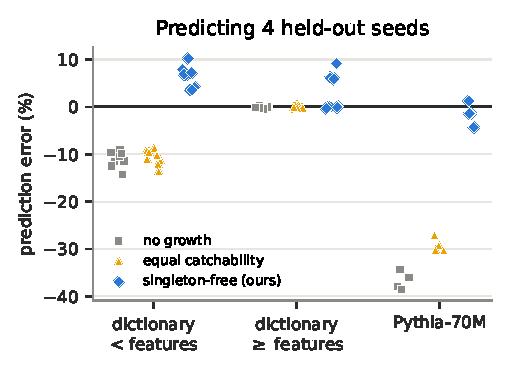
\includegraphics[width=0.55\linewidth]{../figures/fig3_heldout.pdf}
\caption{\textbf{Held-out seeds.} Error in predicting how many features 8 seeds will find at least twice, from 4 seeds. Each point is one setting, averaged over 10 random 4-seed subsets.}
\label{fig:heldout}
\end{figure}

\subsection{When features split}
\label{sec:hier}
Real features are hierarchical: a larger dictionary can replace one coarse feature with several finer ones \citep{bricken2023monosemanticity,leask2025sparse}. So what does the census count? We plant \HierParents{} parent features, each split into \HierC{} children, \HierChildren{} children in all. Whenever a parent is active, exactly one of its children fires. The children are therefore the features that generate the data, and a parent is their shared direction. Siblings have cosine \HierSiblingCos{} with each other and \HierParentCos{} with their parent, so at $\tau=\MainTau$ a latent can match a child or a parent but not both. We train \HierRuns{} SAEs (\SynSeeds{} seeds, $m$ from $N/8$ to $2N$ with $N$ the number of children, \HierDraws{} data draws, other settings unchanged). For the oracle we match latents against both levels (Figure~\ref{fig:hier}).

\begin{figure}[t]
\centering
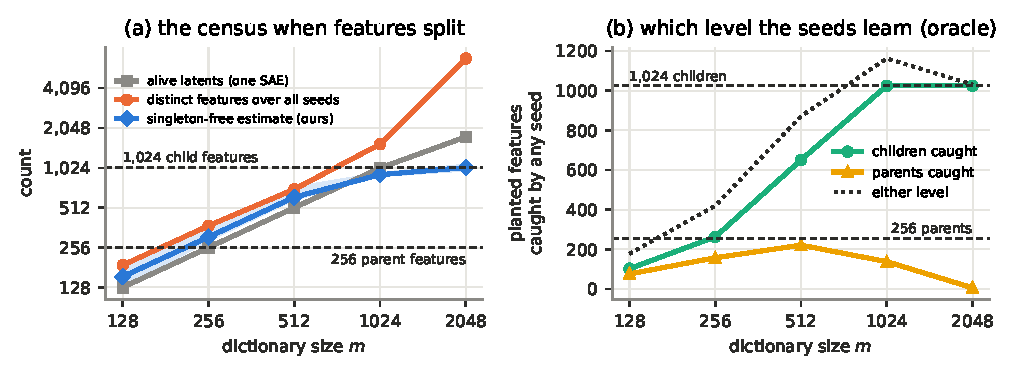
\includegraphics[width=\linewidth]{../figures/fig4_hierarchy.pdf}
\caption{\textbf{Features that split.} \HierParents{} planted parents, each with \HierC{} children (\HierChildren{} in all). (a) Counts against dictionary size, averaged over \HierDraws{} data draws; bands show the range over draws, and for the census the bootstrap intervals of both. The census rises with the dictionary and levels off at the child count only once there is room for every child. (b) Planted features caught by at least one of \SynSeeds{} seeds under oracle matching. Small dictionaries learn a mixture of parents and children.}
\label{fig:hier}
\end{figure}

\paragraph{Small dictionaries do not settle on the coarse level.} At $m=N/4$ there is room for exactly the \HierParents{} parents. Even so, the seeds learn a mixture: under oracle matching, \HierKidsQuarter{} children and \HierParsQuarter{} parents are caught by at least one seed. The census does not stop at \HierParents{}. It rises with the dictionary (\HierSfEighth, \HierSfQuarter{} and \HierSfHalf{} at $m=N/8$, $N/4$ and $N/2$), at \HierSfReachMed{} of the features reachable at either level (median; range \HierSfReachMin--\HierSfReachMax). A coarse level therefore does not create a false plateau.

\paragraph{Once the finest level fits, the census finds it.} At $m=2N$ the estimate is \HierSfDouble{} against \HierChildren{} children. It is within \HierSfErrDouble{} of the child count in both draws and at all three matching thresholds. Over the same seeds, the number of distinct latents reaches \HierUnionDouble{} (\HierUnionRatioMax-fold). For $m\ge N$, a median \HierJunkSingle{} of the features caught by only one seed match no planted feature at either level.

\paragraph{At $m=N$ the census undercounts.} The estimate is \HierSfFull{}, \HierSfErrFull{} below the child count, even though every child is caught by some seed. A likely cause is that the seeds disagree about the level: \HierParsFull{} parents are also caught by at least one seed. A child that only some seeds resolve looks rarer than it is. This setting is also the most sensitive to the threshold (\HierSfFullTauLo{} at $\tau=\TauLo$, \HierSfFullTauHi{} at $\tau=\TauHi$). At $\tau=\TauLo$ a parent latent can match a child latent, since their cosine of \HierParentCos{} clears the threshold. Held-out prediction is also worse with hierarchy. Fitted on four seeds, the singleton-free model overshoots the eight-seed count by a median of \HeldHierSmallSfMed{} for $m<N$ and \HeldHierBigSfMed{} (maximum \HeldHierBigSfMax) for $m\ge N$. ``No growth'' misses by \HeldHierSmallNoGrowthMed{} and \HeldHierBigNoGrowthMed{}.

Splitting changes how a census curve should be read, not whether the census works. At a given dictionary size, the census counts the features that size resolves, and a plateau marks the finest level the dictionaries can hold. On Pythia-70M the count keeps growing (\S\ref{sec:real}). Splitting produces the same growth whenever the finest level does not yet fit, so that growth alone does not show a fixed population larger than the dictionaries we trained.


\subsection{A census of Pythia-70M}
\label{sec:real}

We now count features where the answer is unknown: the residual stream after block \RealLayer{} of Pythia-70M, with \RealSeeds{} seeds at each of four dictionary sizes (Table~\ref{tab:real}, Figure~\ref{fig:hero}b).

\begin{table}[t]
\centering\small
\caption{\textbf{Census of Pythia-70M} (layer \RealLayer, \RealSeeds{} seeds per size, $\tau=\MainTau$). FVU is the fraction of variance unexplained on held-out tokens (mean over seeds). ``Distinct, all seeds'' is the union over seeds. ``Seen $\ge2$'' counts features reproduced by at least two seeds. The interval is a 95\% bootstrap interval for the singleton-free estimate.}
\label{tab:real}
\begin{tabular}{rrrrrrrl}
\toprule
$m$ & FVU & alive & distinct, all seeds & seen $\ge 2$ & Chao $M_h$ & singleton-free & 95\% CI \\
\midrule
1{,}024 & 0.090 & 1{,}024 & 6{,}107 & 543 & 98{,}244 & 870 & [728, 1{,}083] \\
2{,}048 & 0.082 & 2{,}048 & 12{,}900 & 934 & 238{,}236 & 1{,}616 & [1{,}303, 2{,}011] \\
4{,}096 & 0.077 & 4{,}089 & 27{,}515 & 1{,}428 & 705{,}721 & 2{,}520 & [2{,}113, 2{,}941] \\
8{,}192 & 0.073 & 8{,}044 & 57{,}614 & 1{,}867 & 2{,}405{,}854 & 3{,}172 & [2{,}869, 3{,}952] \\
\bottomrule
\end{tabular}

\end{table}

\paragraph{Seeds disagree much more than on planted features.} At $m=8192$, \RealSingleFrac{} of the distinct features found across seeds were found by one seed only, and just \RealAllSeedsEight{} by all eight. The union over seeds grows \RealUnionGrowth-fold from $m=1024$ to $m=8192$, slightly faster than the dictionary itself, and Chao's bound reaches the millions. Both are the junk-driven signatures of the synthetic over-complete regime.

\paragraph{The singleton-free census.} The estimated number of reproducible features grows from \RealSfOne{} (95\% CI \RealSfLoOne--\RealSfHiOne) at $m=1024$ to \RealSfEight{} (\RealSfLoEight--\RealSfHiEight) at $m=8192$. Each doubling of the dictionary multiplies the estimate by \RealGrowthOne, \RealGrowthTwo{} and \RealGrowthFour{}. Growth is slowing, but by the logic of \S\ref{sec:sf} it has not stopped, so these dictionaries have not yet reached the plateau and \RealSfEight{} is a lower bound for this layer under our training budget. At $m=8192$ only about \RealReproFrac{} of a single SAE's alive latents correspond to reproducible features, a regime we did not see with planted features.

\paragraph{Held-out seeds confirm the forecasts.} Fitted on 4 seeds, the singleton-free model predicts how many features all 8 seeds reproduce to within \HeldRealSfMax{} at every dictionary size (median \HeldRealSfMed; Figure~\ref{fig:heldout}). In the median, assuming no new features would appear misses by \HeldRealNoGrowthMed, and assuming equal catchability by \HeldRealMZeroMed. This test needs no ground truth, so it is the strongest evidence that the census describes real structure in the seeds' agreement.

\paragraph{What the census is sensitive to.} The matching threshold matters more for real features than for planted ones (Appendix Table~\ref{tab:real_tau}). At $m=8192$ the estimate is \RealSfEightTauLo{} at $\tau=\TauLo$ and \RealSfEightTauHi{} at $\tau=\TauHi$. The growth with dictionary size holds for $\tau\le\MainTau$, but at $\tau=\TauHi$ the estimate falls between $m=4096$ and $m=8192$. Real features are reproduced less exactly than planted directions, so deciding when two latents are ``the same feature'' is a modelling choice that the count inherits. The number of seeds matters less: at $m=8192$, fitting 4, 6 and 8 seeds gives \RealSfEightKFour, \RealSfEightKSix{} and \RealSfEight.

\paragraph{More training data makes seeds agree, and raises the count.} We retrained the $m=2048$ family on \RealLongTokens{} tokens, five times more data, in one pass (\RealLongStepRatio{} times as many training steps). The model, layer and evaluation set are unchanged. The new SAEs reconstruct better (FVU \RealLongFvu{} vs \RealFvuTwo) and agree more: \RealLongAllSeeds{} features are found by all eight seeds, against \RealAllSeedsTwo. The singleton-free estimate rises from \RealSfTwo{} to \RealLongSf{} (95\% CI \RealLongSfLo--\RealLongSfHi), a factor of \RealLongRatio. Across the three matching thresholds it now ranges only from \RealLongTauMin{} to \RealLongTauMax, against \RealTwoTauMin{} to \RealTwoTauMax{} before, and the held-out prediction from four seeds is off by \RealLongHeldErr. Part of the seed disagreement on Pythia is therefore a training-budget effect. Our census counts are lower bounds in two senses: the dictionaries are too small to plateau, and more training would reveal more reproducible features.



\section{Discussion}
\label{sec:discussion}

\paragraph{What the estimate means.} The singleton-free estimate does not count ``all features a model has''. Capture--recapture cannot answer that, for animals or for features \citep{link2003nonidentifiability}. It counts the features that SAEs of a given size find with probability at least $1/K$ per seed. Two properties make it useful. First, in every synthetic setting where the answer is known and reachable, it is right to within a few percent while all naive counts are badly wrong (Table~\ref{tab:synth}). Second, its behaviour across dictionary sizes is diagnostic. It rises while the dictionary is too small and levels off at the feature count once the dictionary is large enough. A practitioner can therefore read off when a larger SAE stops buying new features, which is the question behind choosing a dictionary size, without any ground truth.

\paragraph{Why seed disagreement is informative.} \citet{paulo2025sparse} showed that seeds disagree. Our results separate two sources of disagreement. Some features are real but rare, so a dictionary too small to hold them all catches different subsets on different seeds. Others are junk directions that a single seed learns. The first kind is structure the census should count. The second is noise it should ignore. The capture-frequency histogram tells them apart, because junk is almost never reproduced.

\paragraph{Limitations.}
\begin{itemize}\setlength\itemsep{1pt}
\item \emph{Synthetic world.} Our main planted features are independent, equally sized random directions with Zipf-like frequencies. Real features are correlated, hierarchical and split as dictionaries grow \citep{bricken2023monosemanticity,leask2025sparse}, which can turn one ``species'' into several. Section~\ref{sec:hier} tests one simple form of splitting, a single parent--child level with fixed geometry. There the census levels off at the finest level only once it fits, and undercounts by \HierSfErrFull{} when the dictionary is just large enough. Real hierarchies are deeper and less regular. The synthetic results show the estimator works when a fixed population exists. They cannot show that one exists in a real model.
\item \emph{Seeds are not independent nets.} All seeds see the same data in the same order, and identification relies on a cosine threshold. We checked $\tau\in\{\TauLo,\MainTau,\TauHi\}$, but correlated failures, such as all seeds merging the same two features, would be invisible to any capture--recapture estimator.
\item \emph{The probability floor defines the target.} With $K$ seeds, features caught with probability well below $1/K$ are out of reach by construction. Halving the floor changed results little in our synthetic settings, but that need not hold elsewhere.
\item \emph{Scale and training budget.} We used dictionaries of at most 8k latents on one layer of a 70M-parameter model, with \RealSeeds{} seeds, trained on \RealTrainTokens{} tokens and checked once with \RealLongTokens{}, on a laptop CPU. More data raised the count, so our Pythia numbers describe SAEs trained on this budget. Frontier SAEs have millions of latents. The method's cost is $K$ training runs, which is significant at that scale.
\item \emph{Few-seed bias.} Fitted to four seeds, the estimator over-predicts what further seeds find by up to about a tenth (\S\ref{sec:heldout}).
\end{itemize}

\paragraph{Broader impact.} This is a measurement tool for interpretability research. Knowing how many features a model has, or that a dictionary has stopped finding new ones, helps decide how much of a model an interpretability method has actually covered. That matters when SAE features are used to audit model behaviour. A risk is false reassurance: a plateau means an SAE family stopped finding \emph{reachable} features, not that the model has no others. We see no direct path to misuse.



\bibliographystyle{plainnat}
\bibliography{refs}

\appendix
\section{Estimators in detail}
\label{app:estimators}

Throughout, $K$ is the number of seeds, $Y_s\in\{0,\dots,K\}$ the number of seeds that catch species $s$, $Q_j=\#\{s: Y_s=j\}$, $S=\sum_{j\ge1}Q_j$ and $S_{\ge2}=\sum_{j\ge2}Q_j$. Under model $M_h$ each species has its own catch probability $p_s$, drawn from an unknown distribution $G$, and seeds catch independently given $p_s$. Then $Y_s\mid p_s\sim\mathrm{Binomial}(K,p_s)$ and
\begin{equation}
\mathbb E\,Q_j = N\binom{K}{j}\mu_j,\qquad \mu_j=\int p^j(1-p)^{K-j}\,dG(p).
\end{equation}

\paragraph{Why Chao's estimator is a lower bound.} By Cauchy--Schwarz, $\mu_1^2=\big(\int p^{1/2}(1-p)^{K/2}\cdot p^{1/2}(1-p)^{(K-2)/2}\,dG\big)^2\le\mu_0\,\mu_2$. Substituting expected counts gives $\mathbb E Q_0\ge\frac{K-1}{K}\,(\mathbb EQ_1)^2/(2\,\mathbb EQ_2)$, the bound of \citet{chao1987estimating}. The bound is tight when $G$ is a point mass and loose when $G$ has mass near zero. It is also \emph{increasing} in $Q_1$, so every spurious singleton that blind matching creates inflates it quadratically. That is the failure in Table~\ref{tab:synth}.

\paragraph{Jackknife.} The first- and second-order jackknives of \citet{burnham1978estimation} are $S+\frac{K-1}{K}Q_1$ and $S+\frac{2K-3}{K}Q_1-\frac{(K-2)^2}{K(K-1)}Q_2$. They are linear in $Q_1$, so they are inflated less violently than Chao's bound, but still inflated.

\paragraph{Lincoln--Petersen and $M_t$.} For seeds $a,b$ with $n_a,n_b$ captures and $m_{ab}$ species caught by both, Chapman's estimator is $(n_a+1)(n_b+1)/(m_{ab}+1)-1$ \citep{chapman1951some}. We average it over all $\binom K2$ pairs. The $M_t$ maximum-likelihood estimate solves $\prod_r(1-n_r/N)=1-S/N$ \citep{darroch1958multiple}. Both assume equal catchability and undercount when it fails.

\paragraph{Singleton-free mixtures.} Conditioning on $Y\ge2$ removes $Q_0$ and $Q_1$ from the likelihood:
\begin{equation}
\ell(\theta)=\sum_{j=2}^{K}Q_j\Big[\log\pi_j(\theta)-\log\textstyle\sum_{i\ge2}\pi_i(\theta)\Big],\qquad \pi_j(\theta)=\binom Kj\mu_j(\theta),
\end{equation}
which we maximise with Nelder--Mead from several starting points, and we set $\hat N=S_{\ge2}/\sum_{i\ge2}\pi_i(\hat\theta)$. The mixing distribution $G$ is a $c$-point mixture \citep{pledger2000unified}, $c\in\{1,2,3\}$, with $2c-1$ parameters, with support points in $[p_{\min},1)$ and $p_{\min}=1/K$. The reported estimate comes from the $c$ with the lowest AIC, $-2\ell+2(2c-1)$.

Both choices matter, and the ablation rows of Table~\ref{tab:synth} show what goes wrong without them. Without the lower bound, a beta or two-point $G$ can place mass near $p=0$ while barely changing the truncated likelihood, because such species are almost never caught twice. The maximum-likelihood estimate then sits on the boundary with $\hat N\to\infty$. This happened in the over-complete runs: a single species caught by five of eight seeds, next to a thousand caught by all eight, was enough. That is Link's non-identifiability \citep{link2003nonidentifiability} in its most practical form. The bound turns ``how many features exist'' into the identifiable question ``how many features does a seed find with probability at least $1/K$''. Without AIC, a superfluous class can absorb noise. When an estimate exceeds $10^9$ we report it as diverged (``div.'').

\paragraph{Predicting more seeds.} With $\hat\theta$ and $\hat N$ from $K'$ seeds, the expected number of species caught at least twice by $K$ seeds is $\hat N\sum_{j\ge2}\binom Kj\mu_j(\hat\theta;K)$. The held-out experiment compares this with the count blind matching finds among all $K$ seeds.

\paragraph{Bootstrap.} Given $\hat N$, we append $\hat N-S$ all-zero rows to $H$, resample $\hat N$ rows with replacement, drop the zero rows, and recompute the estimator. Intervals are the 2.5th and 97.5th percentiles of \BootN{} resamples.

\section{Experimental details}
\label{app:details}

\paragraph{SAE.} TopK SAE \citep{gao2024scaling}: $z=\mathrm{TopK}(W_{\rm enc}^\top(x-b_{\rm dec})+b_{\rm enc})$ followed by ReLU, and $\hat x=W_{\rm dec}^\top z+b_{\rm dec}$. Decoder rows are kept at unit norm, with the component of each gradient parallel to its row removed. The encoder is initialised as the transpose of the decoder, and $b_{\rm dec}$ as the mean of the first batch. A latent is dead if it has not fired for 200k samples, and the AuxK loss (coefficient $1/32$, $k_{\rm aux}=\min(m/2,2k)$) reconstructs the residual from the top dead latents. Optimiser: Adam with $\beta=(0.9,0.999)$, constant learning rate, then linear decay to zero over the last 20\% of steps; batch size 4096. Seed $s$ seeds only the initialisation, from a random stream disjoint from every synthetic-data stream. (An early version shared the stream, so one seed's initialisation \emph{was} the planted dictionary. A test now guards against this.)

\paragraph{Synthetic data.} Features $f_i\sim\mathrm{Uniform}(S^{d-1})$ with $d=\SynD$. Feature $i$ fires with probability $p_i=\min(1,c\,i^{-\SynAlpha})$, with $c$ set so that $\sum_ip_i=\SynMeanActive$, and with magnitude $U(0.5,1.5)$. Training data are 400 batches of 4096 samples, materialised once and reused for three passes (\SynSteps{} steps). Evaluation uses 16{,}384 samples from a disjoint random stream. Settings: $N\in\{512,1024,2048\}$; $m/N\in\{1/4,1/2,1,2,4\}$ with $m\le4096$, except $(N,m)=(2048,4096)$; plus a second feature/data draw for $N=1024$, $m/N\le2$. That gives \SynFamilies{} settings and \SynRuns{} SAEs. TopK $k=\SynK$, learning rate $2\times10^{-3}$.

\paragraph{Hierarchical data (\S\ref{sec:hier}).} For each of the \HierParents{} parents we draw $\HierC+1$ orthonormal directions $g,u_1,\dots,u_{\HierC}$ (QR of a Gaussian matrix) and set child $j$ to $0.6\,g+0.8\,u_j$, so siblings have cosine exactly \HierSiblingCos{}. The parent reference is the normalised mean of its children, at cosine \HierParentCos{} to each. Parent $i$ fires with probability $\min(1,c\,i^{-\SynAlpha})$, with $c$ set so that $\sum_ip_i=\SynMeanActive$. When it fires, one of its children, chosen uniformly, takes magnitude $U(0.5,1.5)$. We use $d=\SynD$, $N=\HierChildren$ children, $m\in\{N/8,N/4,N/2,N,2N\}$ and \HierDraws{} data draws with \SynSeeds{} seeds each, with all other settings as above. Oracle matching uses the children and the parents together as references.

\paragraph{Pythia-70M.} Residual stream after block \RealLayer{} of \texttt{EleutherAI/pythia-70m} (revision \texttt{main}), from 128-token contexts of \texttt{NeelNanda/pile-10k} \citep{pile10k}. Documents are concatenated with an end-of-text token between them, and the first position of each context is dropped. There are \RealTrainTokens{} training tokens (documents 500 onward, shuffled once with a fixed seed) and \RealEvalTokens{} evaluation tokens (documents 0--499). Activations are scaled by one global constant so that $\mathbb E\|x\|^2=d$ and stored in float16. TopK $k=\RealK$, learning rate $10^{-3}$ (chosen over $3\times10^{-4}$ by evaluation FVU in a one-seed pilot at $m=2048$), two passes over the data.

\paragraph{Matching.} A latent is alive if it fires on at least $10^{-5}$ of evaluation samples. For each pair of runs we compute decoder cosine similarities and link mutual nearest neighbours above $\tau$. Species are the connected components of the union of links over all pairs. Oracle matching (synthetic only) marks planted feature $i$ caught by run $r$ when some alive latent of $r$ has cosine at least $\tau$ with $f_i$.

\paragraph{Compute.} Everything ran on one laptop CPU (AMD Ryzen 7 8845HS, 8 cores, 13\,GB RAM) with no GPU. The synthetic SAEs took about an hour, caching Pythia-70M activations about an hour, and the Pythia-70M SAEs (pilot, main grid and the 10M-token family) a little over two hours. The first analysis pass, with bootstrap intervals, takes about half an hour; later builds reuse its cache and finish in minutes. The hierarchical grid (\S\ref{sec:hier}) took about 80 minutes, slowed by an unrelated job sharing the CPU, and its analysis about 7 minutes. In total the experiments took about six and a half hours. \texttt{build.sh} reruns everything and skips finished runs.

\paragraph{Correctness tests.} \texttt{tests/test\_pipeline.py} plants known answers and checks that each stage recovers them:
\begin{itemize}\setlength\itemsep{0pt}
\item equal-catchability estimators recover $N$, and the bootstrap interval covers it;
\item under heterogeneity, Chao's bound beats $M_t$;
\item 3000 planted junk singletons leave the singleton-free estimate unchanged while Chao's bound explodes;
\item a single stray recapture does not make the bounded estimator diverge;
\item rarefaction identities hold;
\item blind matching recovers a shuffled copy of a dictionary;
\item one SAE recovers nearly all planted features in an easy regime;
\item in the hierarchical data, the two levels are separable at $\tau=\MainTau$: oracle matching of the parent directions catches exactly the parents, and of the child directions exactly the children; at most one child per parent is active.
\end{itemize}

\begin{table}[h]
\centering\small
\caption{Pythia-70M: singleton-free estimate at three matching thresholds, and the number of features all \RealSeeds{} seeds share.}
\label{tab:real_tau}
\begin{tabular}{rrrrr}
\toprule
$m$ & $\tau=0.7$ & $\tau=0.8$ & $\tau=0.9$ & seen by all seeds ($\tau=0.8$) \\
\midrule
1{,}024 & 991 & 870 & 673 & 96 \\
2{,}048 & 1{,}543 & 1{,}616 & 1{,}123 & 167 \\
4{,}096 & 2{,}967 & 2{,}520 & 1{,}543 & 247 \\
8{,}192 & 4{,}254 & 3{,}172 & 1{,}238 & 308 \\
\bottomrule
\end{tabular}

\end{table}



\end{document}
